\chapter{Microservizio anagrafica}\label{cap:microservizio-anagrafica}

\section{Scopo del sistema}

Il sistema di anagrafica si occupa di gestire le informazioni anagrafiche dei sensori, delle aree e dei lampioni. Gestisce questi raggruppamenti e si occupa di renderli persistenti su database.

\section{Requisiti coperti dal sistema}

\subsection{RF\_03}
RF\_03:deve essere possibile aggiungere nuovi sensori a sistema.

Questo microservizio, copre il requisito peristendo i dati anagrafici del sensore.

\subsection{RF\_08}
RF\_08:l'utente deve poter inserire la locazione geografica del sensore nel sistema.

Questo microservizio, copre il requisito peristendo i dati di locazione del sensore.

\subsection{RF\_09}
RF\_09:l'utente deve poter inserire il raggio di azione del sensore.

Questo microservizio, copre il requisito peristendo i dati di raggio di azione del sensore.

\subsection{RF\_10}
RF\_10:l'utente deve poter essere in grado di visualizzare quali aree sono illuminate in un dato momento

Questo microservizio, copre parte del requisito fornendo l'informazione di quali lampioni si trovano in una determinata area.



\section{Descrizione del sistema}

Il sistema principalmente fornisce le informazioni stoccate su base dati tramite un'interfaccia rest.
Questo è poi in grado di fornire i dati in forma aggregata, come ad esempio il numero di lampioni per area, o il numero di sensori per lampioni.

Per queste informazioni ha inoltre il compito e la responsabilità di tenere aggiornati i dati nel database.

\section{Architettura del sistema}

L'architettura base del sistema è in MVVM perché non è presente la necessità di multi input e multi output e un'architettura di altro tipo avrebbe aggiunto complessità inutile al sistema.

I componenti del programma sono quindi divisi in tre parti: Model, View e ViewModel.

\begin{figure}[h]
    \centering
    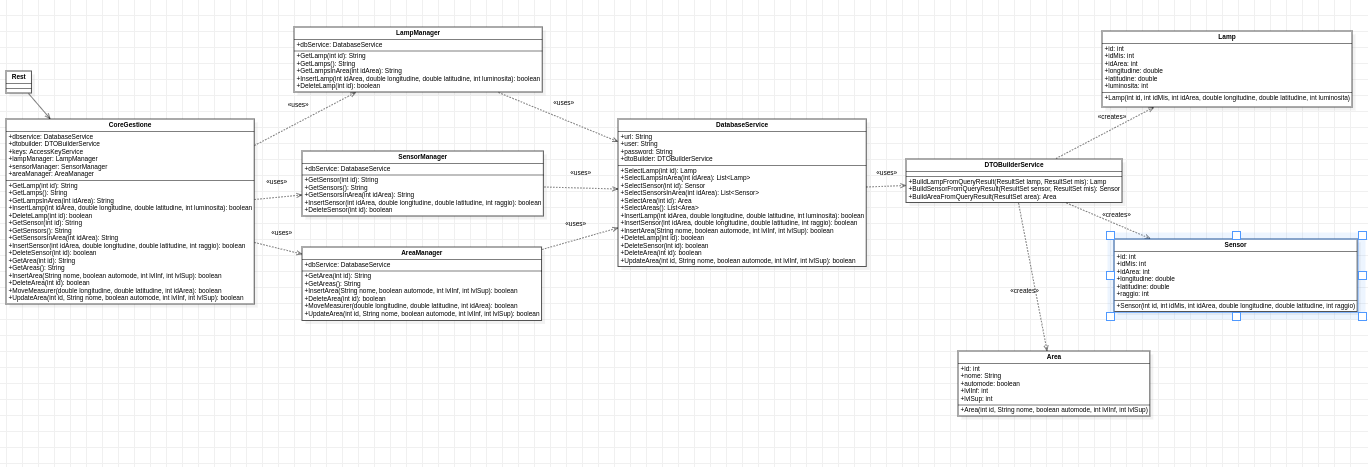
\includegraphics[width=\textwidth]{img/anagrafe_generale.png}
    \caption{Vista generale del sistema di anagrafe}
    \label{fig:general_anagrafe}
\end{figure}

\section{Model}
\begin{figure}[h]
    \centering
    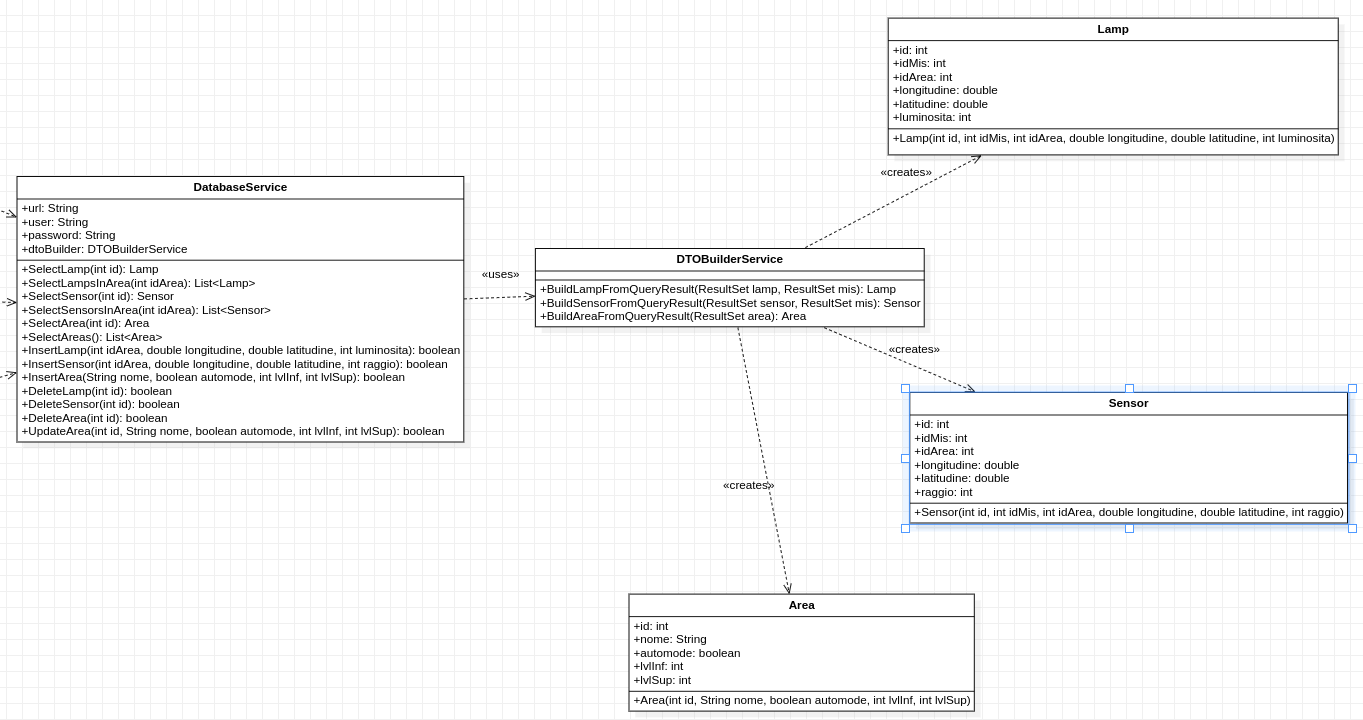
\includegraphics[width=\textwidth]{img/model_anagrafe.png}
    \caption{Diagramma delle classi del modello all'interno del sistema di anagrafe}
    \label{fig:model_anagrafe}
\end{figure}

\begin{itemize}
    \item \textbf{LampManager}: si occupa della gestione (ottenimento, inserimento, modifica o cancellazione) dei dati relativi ai lampioni nel database.
    \item \textbf{SensorManager:} si occupa della gestione (ottenimento, inserimento, modifica o cancellazione) dei dati relativi ai sensori nel database. 
    \item \textbf{AreaManager:} si occupa della gestione (ottenimento, inserimento, modifica o cancellazione) dei dati relativi alle aree nel database.
\end{itemize}

\section{Port Interfaccia REST}

L'interfaccia rest viene esposta all'esterno e permette di effettuare le operazioni discusse nelle sotto-sezioni successive.

\begin{itemize}
    \item GET /getLamp/id
    \item GET /getLampsInArea/idArea
    \item PUT /addLamp
    \item PUT /deleteLamp/id
    \item GET /getSensor/id
    \item GET /getSensorsInArea/idArea
    \item PUT /addSensor
    \item PUT /deleteSensor/id
    \item PUT /moveMeasurer/idMeasurer
    \item GET /getArea/id
    \item GET /getAreaList
    \item PUT /addArea
    \item PUT /updateArea/id
    \item PUT /deleteArea/id
\end{itemize}

\subsection{ GET /getLamp/id}

GetLamp permette di ottenere tutti i dati relativi a un lampione. L'utente deve fornire l'id del lampione in questione.

Il sistema risponderà con un JSON contenente tutti i dati relativi al lampione richiesto.

\subsection{ GET /getLampsInArea/idArea}

GetLampsInArea permette di ottenere i dati relativi a tutti i lampioni in un'area. L'utente deve fornire l'id dell'area della quale si desidera visualizzare i lampioni.

Il sistema risponderà con un JSON contenente tutti i dati relativi ai lampioni presenti in quell'area.

\subsection{ PUT /addLamp}

AddLamp permette di inserire nel database un nuovo lampione. All'utente è richiesto di fornire i dati relativi al lampione da inserire in un JSON che viene inviato al sistema.

Il sistema risponderà con un boolean ad indicare se l'operazione è andata a buon fine o meno.

\subsection{ PUT /deleteLamp/id}

DeleteLamp permette di eliminare dal database un lampione. L'utente deve fornire al sistema l'id del lampione da eliminare.

Il sistema procede poi a tentare di eliminare il lampione, rimuovendo prima il riferimento al misuratore, e ritorna un boolean positivo in caso di successo, negativo in caso di fallimento.

\subsection{ GET /getSensor/id}

GetSensor permette di ottenere tutti i dati relativi a un sensore. L'utente deve fornire l'id del sensore in questione.

Il sistema risponderà con un JSON contenente tutti i dati relativi al sensore richiesto.

\subsection{ GET /getSensorsInArea/idArea}

GetSensorsInArea permette di ottenere i dati relativi a tutti i sensorioni in un'area. L'utente deve fornire l'id dell'area della quale si desidera visualizzare i sensorioni.

Il sistema risponderà con un JSON contenente tutti i dati relativi ai sensorioni presenti in quell'area.

\subsection{ PUT /addSensor}

AddSensor permette di inserire nel database un nuovo sensore. All'utente è richiesto di fornire i dati relativi al sensore da inserire in un JSON che viene inviato al sistema.

Il sistema risponderà con un boolean ad indicare se l'operazione è andata a buon fine o meno.

\subsection{ PUT /deleteSensor/id}

DeleteSensor permette di eliminare dal database un sensore. L'utente deve fornire al sistema l'id del sensore da eliminare.

Il sistema procede poi a tentare di eliminare il sensore, rimuovendo prima il riferimento al misuratore, e ritorna un boolean positivo in caso di successo, negativo in caso di fallimento.

\subsection { PUT /moveMeasurer/id}

MoveMeasurer permette di spostare un misuratore (che può essere un lampione o un sensore) da un'area a un'altra. L'utente deve fornire l'id del misuratore da spostare e un JSON contenente le nuove coordinate e l'area dove va inserito.

Il sistema ritorna infine un boolean positivo in caso di successo, negativo in caso di fallimento.


\section{ViewModel}

\section{View}


